\documentclass[a4paper]{article}

\usepackage[english]{babel}
\usepackage[utf8]{inputenc}
\usepackage{amsmath}
\usepackage{graphicx}
\usepackage[colorinlistoftodos]{todonotes}
\usepackage{fullpage}

\title{Data Oriented Gateway Engine}

\author{Mark Bunney, Jr \\ David Buchman}

\date{\today}

\begin{document}
\maketitle

\section{Summary}

The goal of this project is to develop a framework for managing and testing a network of wireless sensors. The components of the network will be encapsulated so that a user can easily test different aspects such as topology, traffic management, and communication protocol. 

\subsection{Hardware}

Two types of nodes were developed for this project: the BoosterPack Node and the Leaf Node. The BoosterPack Node is based on Texas Instrument's CC110L RF BoosterPack kit and uses a 915MHz radio along with an optional 2.4GHz radio. The Leaf Node is a custom board with an LPC812 microcontroller and 2.4GHz radio. Both nodes include a temperature sensor.

To assist in adding new nodes to the network, two smaller boards were made to provide power and environmental sensors. The Power Subboard provides a 3.3V supply derived from USB, single-cell LiPo battery, or a coin cell. The three power sources are hot-swappable and the current power source is represented by two open-drain outputs. Hardware-based undervoltage LiPo protection and charge circuit are also included.

The Sensor Subboard integrates several common sensors into a small package. It includes pressure, altitude, temperature, relative humidity, ambient light, IR light, UV index, and a microphone with digitally controlled amplifier. The sensors share the same I2C bus and all interrupt pins are broken out to the breadboard-compatible header.

\subsection{Software}

Currently the network is managed from an Intel Edison board with both a 915MHz and 2.4GHz radio. An Arduino sketch interfaces with the radios and posts its data to a Python thread via shared memory. The data is formatted and sent over a socket to a webserver running on Edison. The webserver is able to plot certain aspects of the network in real time.

\begin{figure}
\centering
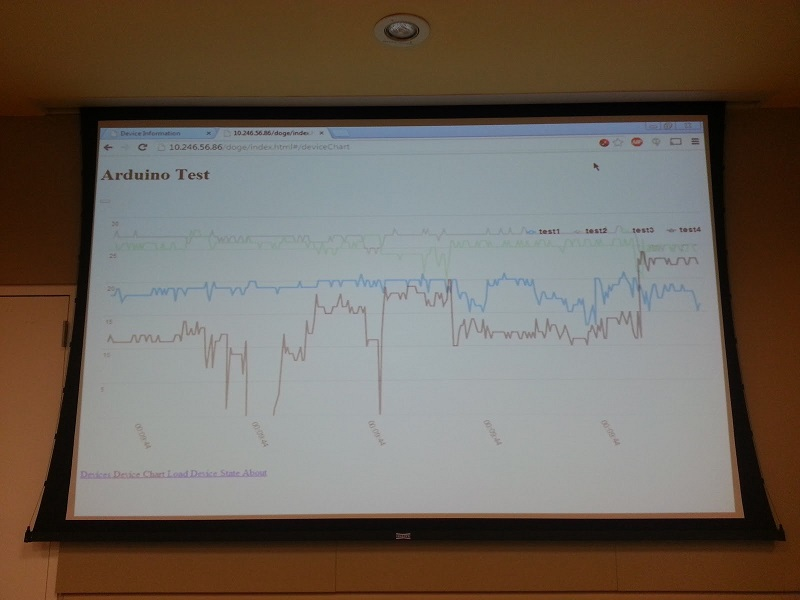
\includegraphics[width=1.0\textwidth]{demo_log.jpg}
\caption{\label{fig:demoLog}Plot of signal strength from 4 915MHz nodes over time via the webserver.}
\end{figure}


\begin{figure}
\centering
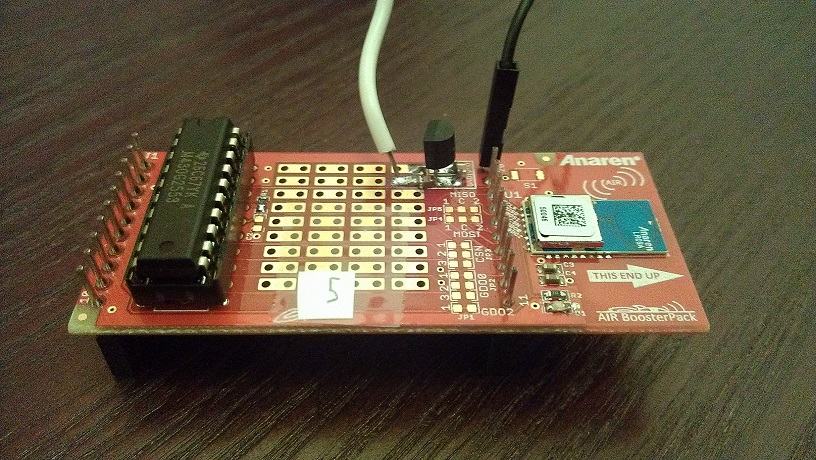
\includegraphics[width=1.0\textwidth]{boosterpack_node.jpg}
\caption{\label{fig:boosterpackNode}MSP430, 3.3V LDO, temperature sensor, and 915MHz radio.}
\end{figure}

\begin{figure}
\centering
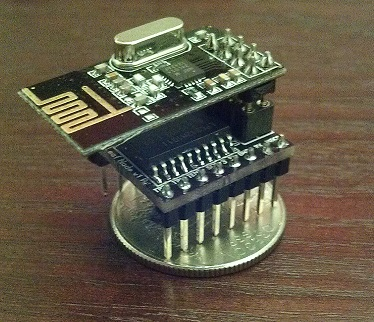
\includegraphics[width=0.7\textwidth]{leaf_node.jpg}
\caption{\label{fig:leafNode}LPC812, temperature sensor, and 2.4GHz radio.}
\end{figure}


\begin{figure}
\centering
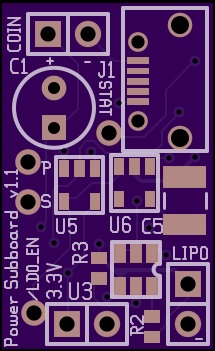
\includegraphics{power_subboard.jpg}
\caption{\label{fig:powerSubboard}Power Subboard}
\end{figure}

\begin{figure}
\centering
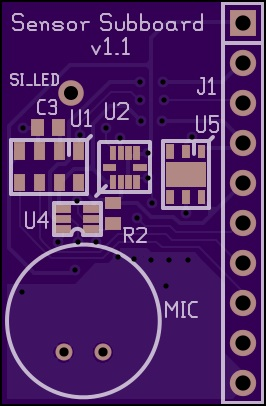
\includegraphics{sensor_subboard.jpg}
\caption{\label{fig:sensorSubboard}Sensor Subboard}
\end{figure}


\end{document}